\section {Approach}

We implemented two commenting systems. The first commenting system is MindMargin with anchored comments on a horizontal infinite scroll next to the reference medium. The second commenting system is a traditional vertical interface.

The client interfaces consist of clean user interfaces to avoid design clutter and distraction. Figure \ref{fig:frontend} shows the MindMargin system in action. The application is split into two sides: The reference media on the left and and an adjacent commenting system on the right. The commenting system displays comments in a horizontal infinite scroll. Thus, an unrestricted amount of comments can be linked to the reference media. Navigation within the infinite scroll component can be performed via mousewheel interaction (either left/right or top/down scrolling with the same effect) or by adjustment of a slider on the bottom of the right split screen. 

Comments are anchored to the horizontal reference point of the media by thin dotted lines. If a comment has replies, a dropdown button appears on the comment's footer. Lighter in color, replies to comments appear vertically under their comment when the button is clicked. This arrangement optimizes horizontal real estate by reserving horizontal space for parent comments. Finally, while navigating through the infinite scroll, the reference medium remains fixed on the left for quick reference against referential comments and replies.

We have also implemented a metric to distinguish between popular and regular comments that appear separately. For greater visibility, popular comments are displayed directly adjacent to the article in the MindMargin interface and directly under the text, or first, in the traditional layout. Upvotes and downvotes indicate and impact comment popularity. 
   
\marginpar{
\begin{figure}
  \begin{center}
  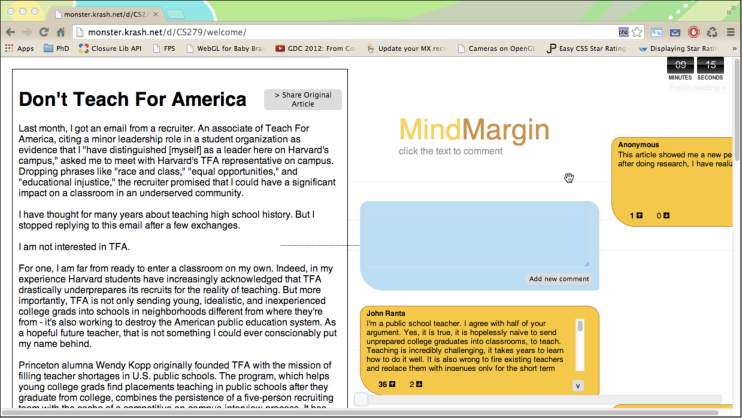
\includegraphics[width=\marginparwidth]{mindmargin.png}
  \caption{The MindMargin system consists of a web client (shown here) and a server side back-end.}
  \label{fig:frontend}
  \end{center}
\end{figure}
}
   
Figure \ref{fig:traditional} shows our implementationof the traditional vertical commenting system. The reference media appears first and on top of the commenting system that follows below. Navigation within the article as well as within the comments can be performed via top/down scrolling. The organization of replies and up- and down-voting is similar to the MindMargin prototype.

\marginpar{
\begin{figure}
  \begin{center}
  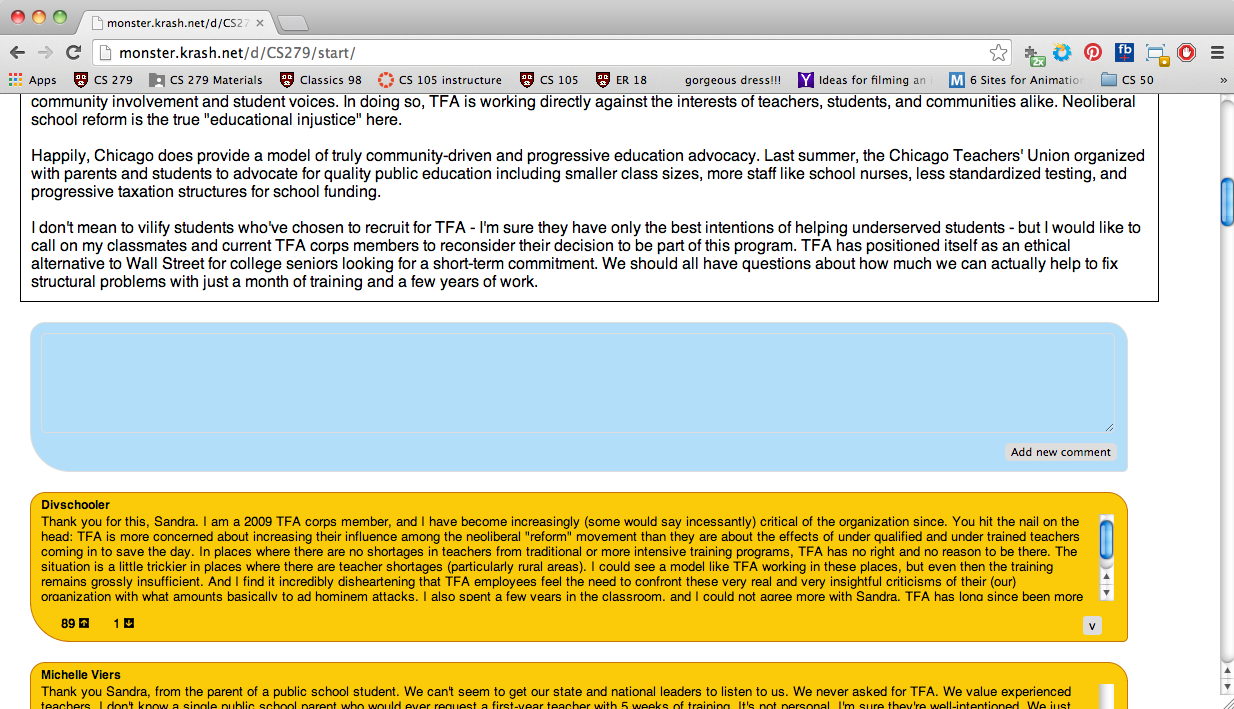
\includegraphics[width=\marginparwidth]{traditional.png}
  \caption{The traditional comment system with a vertically ordered design.}
  \label{fig:traditional}
  \end{center}
\end{figure}
}